\begin{frame}{Learning Rate}
	\begin{itemize}
		\item Learning rate is a hyper-parameter that controls how much we are adjusting the weights of our network with respect the loss gradient. 
	\end{itemize}    
	\begin{figure}[H]
		\centering
		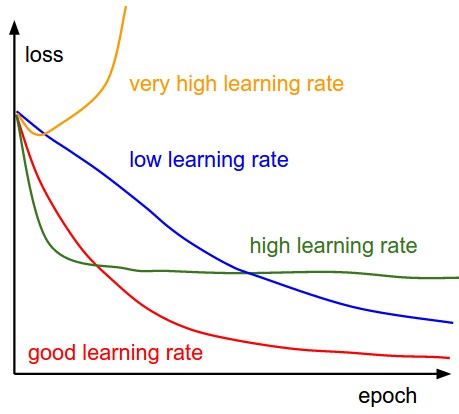
\includegraphics[width=0.4\textwidth]{Figs/lr.png}
		\caption{Learning Rate Effect, \href{https://medium.com/iitg-ai/into-the-depths-of-gradient-descent-52cf9ee92d36}{Source}}
	\end{figure}
\end{frame}

\begin{frame}{Learning Rate}
	\begin{itemize}
		\item Low learning rate 
		\begin{itemize}
			\item Not missing Local Minima.
			\item But takes too much time to converge!
		\end{itemize}
		\item High learning rate 
		\begin{itemize}
			\item Fast, But may diverge!
		\end{itemize}
	\end{itemize}  
	\begin{figure}
		\centering
		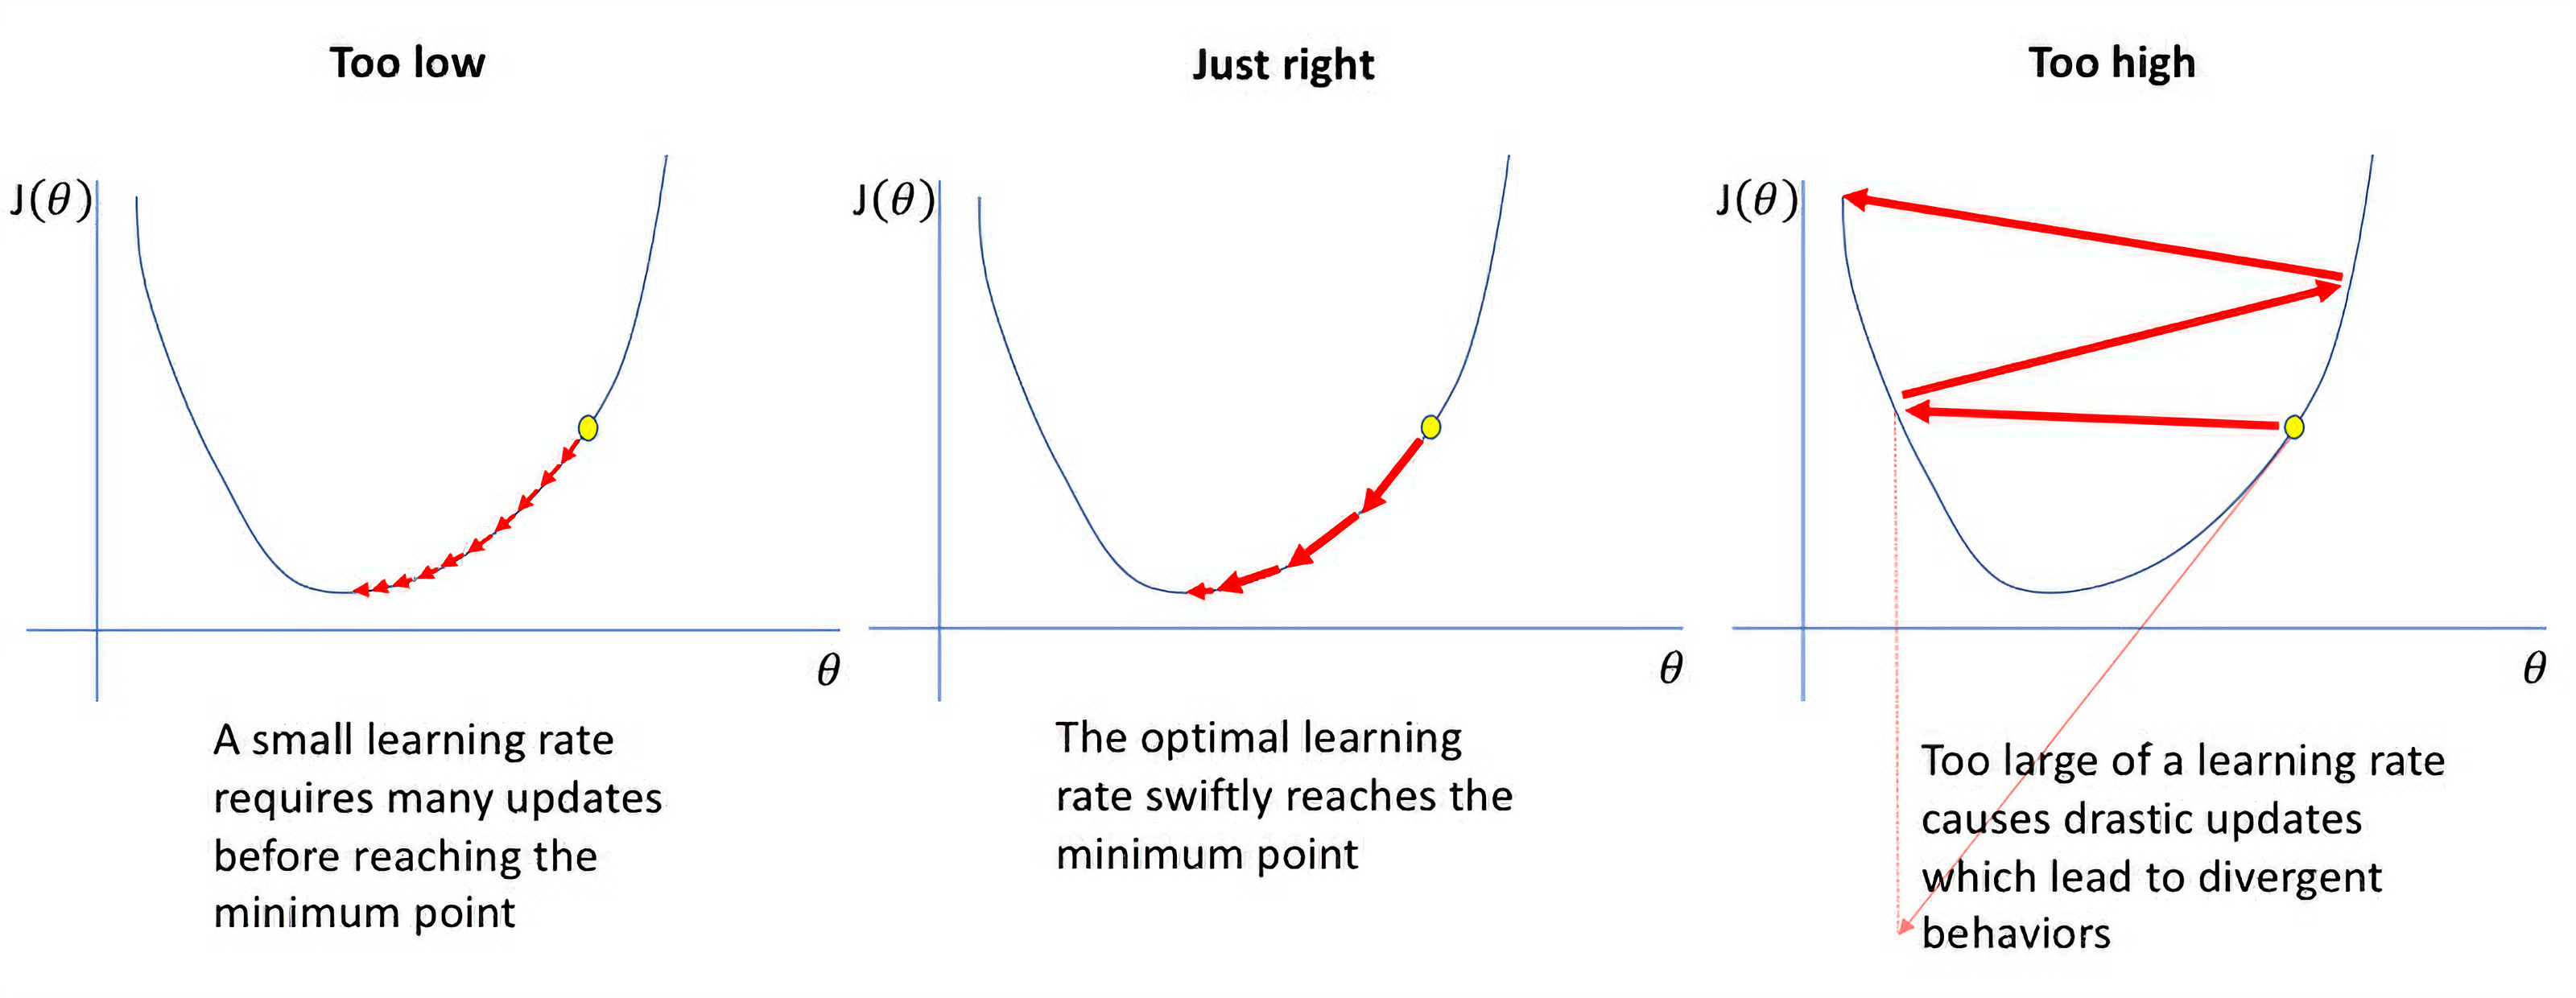
\includegraphics[width=10cm, height=4cm]{Figs/lr_high_res.jpg}
		\caption{Learning Rate Effect, \href{https://www.jeremyjordan.me/nn-learning-rate/}{Source}}
	\end{figure}
\end{frame}

\begin{frame}{Learning Rate}
	\begin{figure}[H]
		\centering
		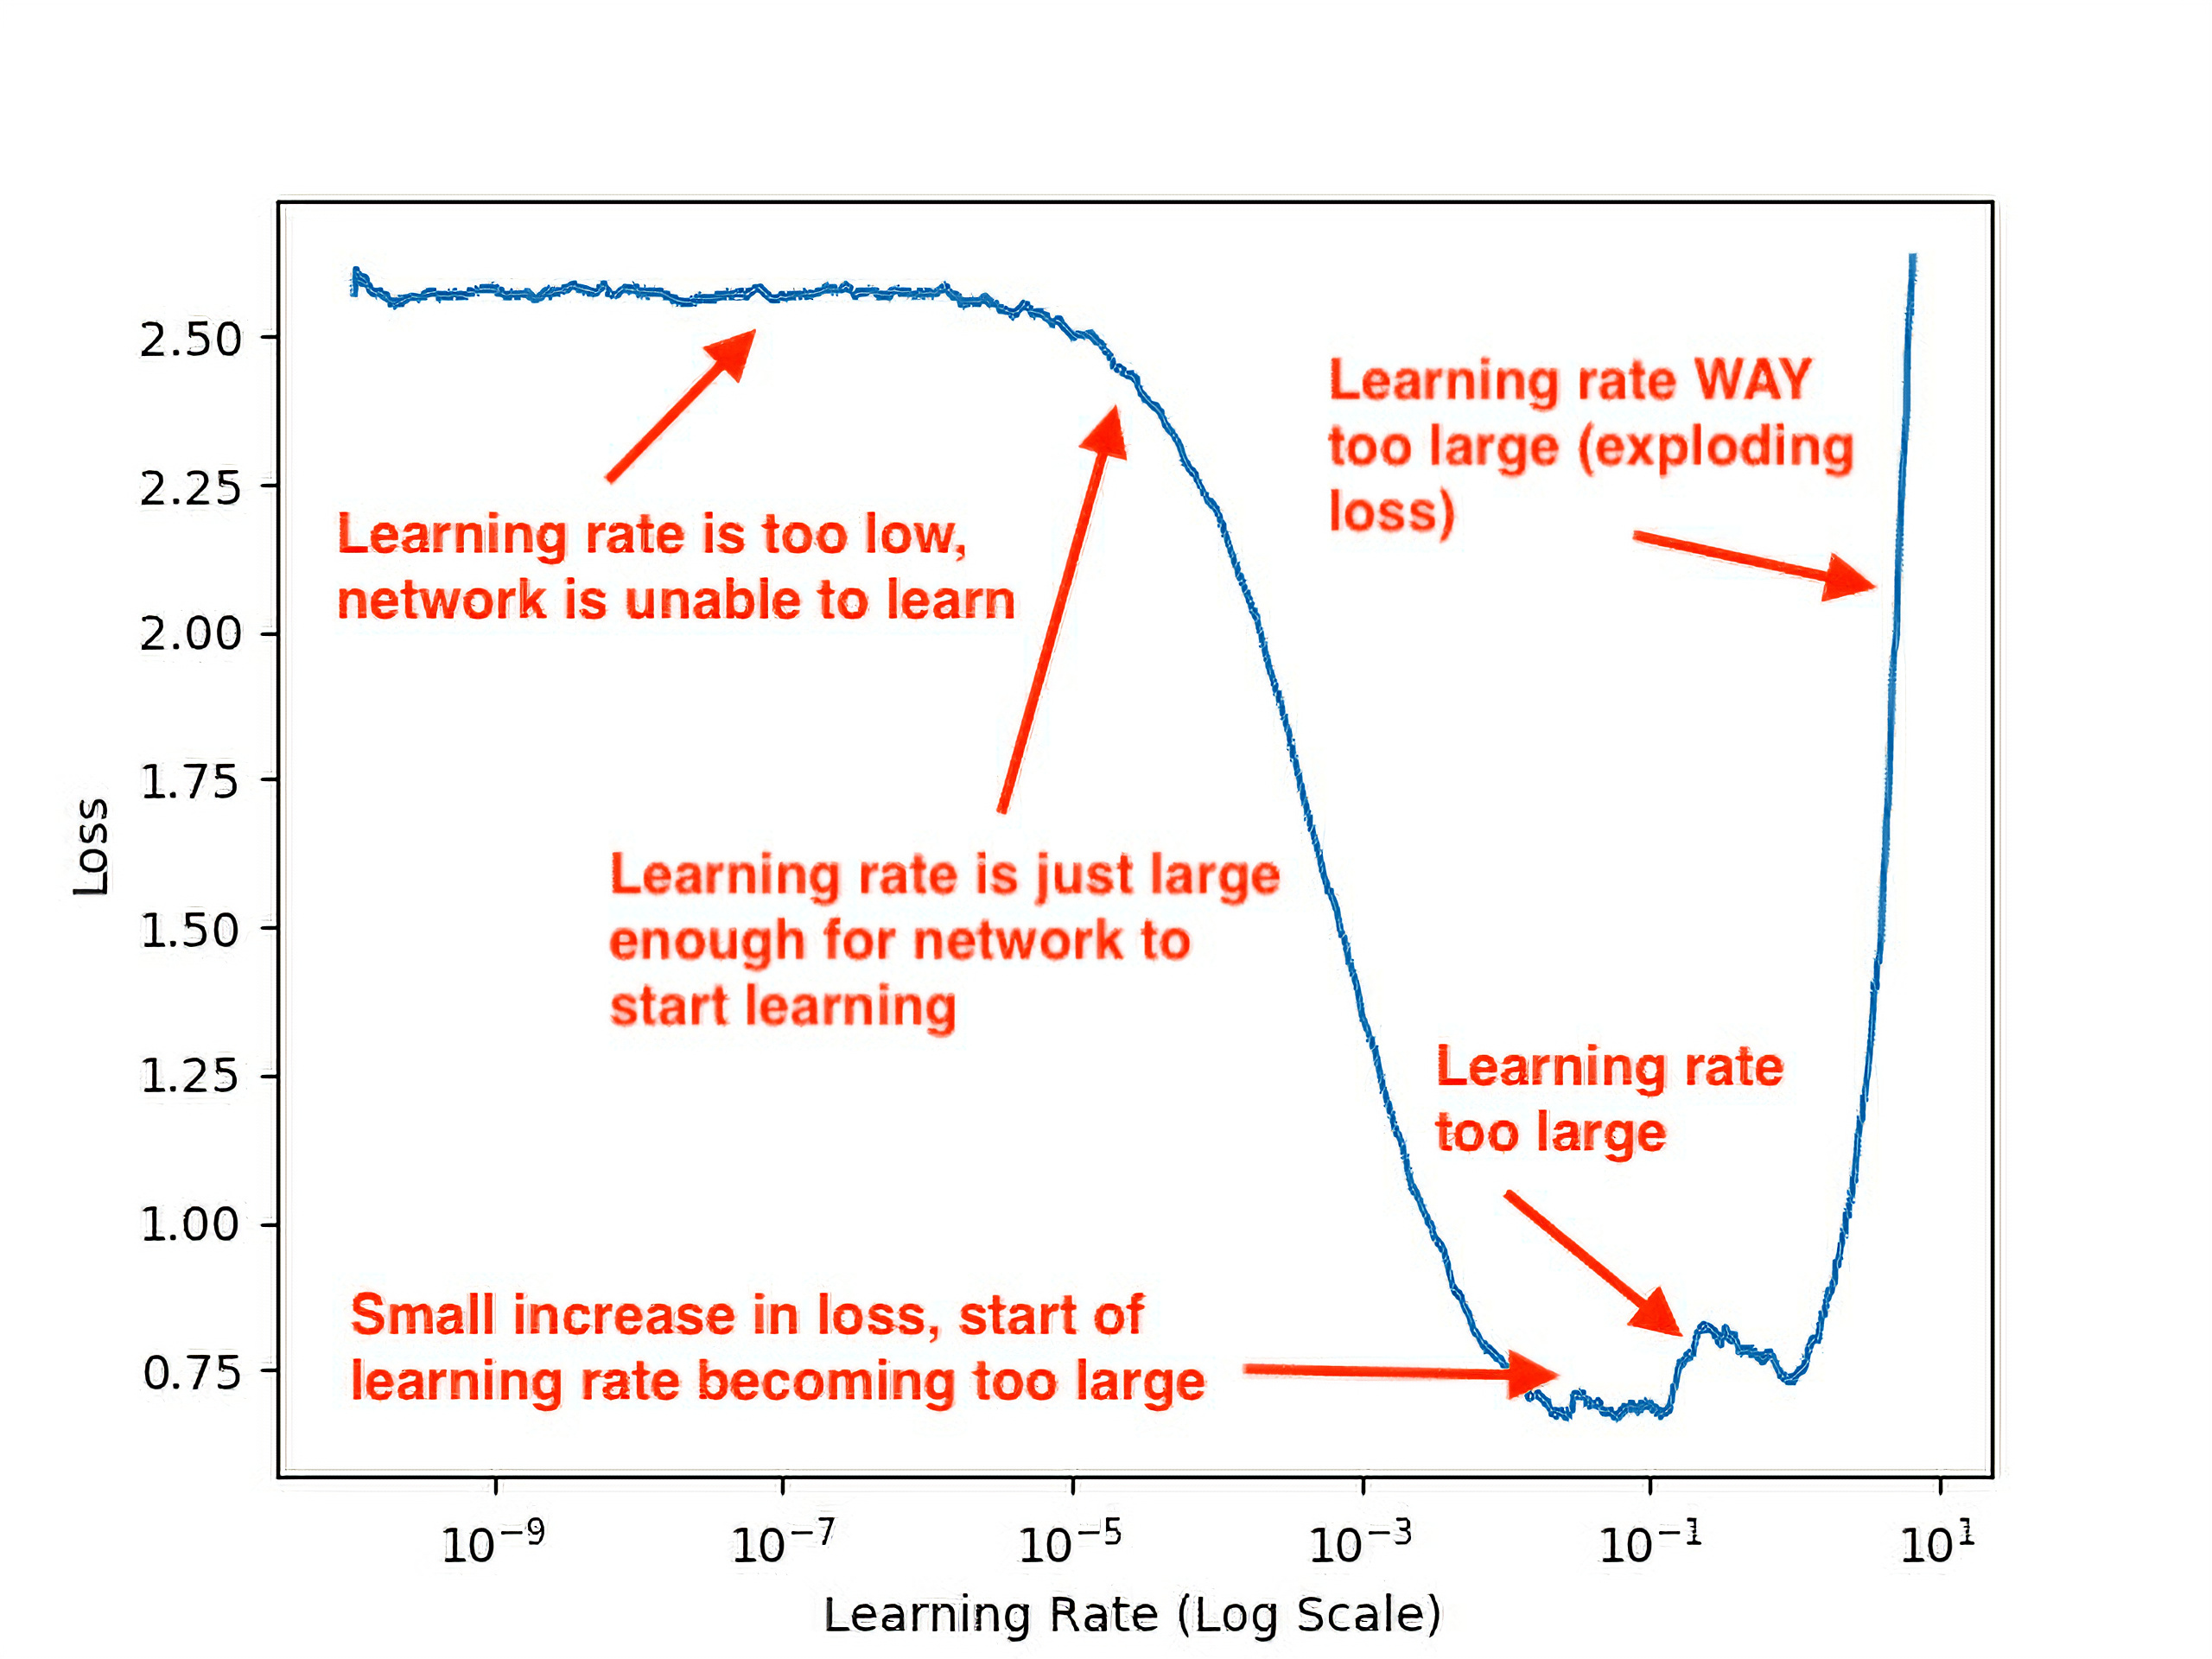
\includegraphics[width=0.7\textwidth]{Figs/lr_high_res_2.jpg}
		\caption{Learning Rate Effect, \href{https://pyimagesearch.com/2019/08/05/keras-learning-rate-finder/}{Source}}
	\end{figure}
\end{frame}